\chapter{Fundamentals}\label{ch:fundamentals}
In this chapter should be explained how the used sensors work, which data they collect and how these data can be used for the purposes of mobile thermal mapping systems.
Furthermore the principals of localization and map creating with help of these sensors are discussed.

\section{Localization and Mapping}\label{sec:localizationAndMapping}

\begin{wrapfigure}[21]{I}{0.60\textwidth}
    \centering
    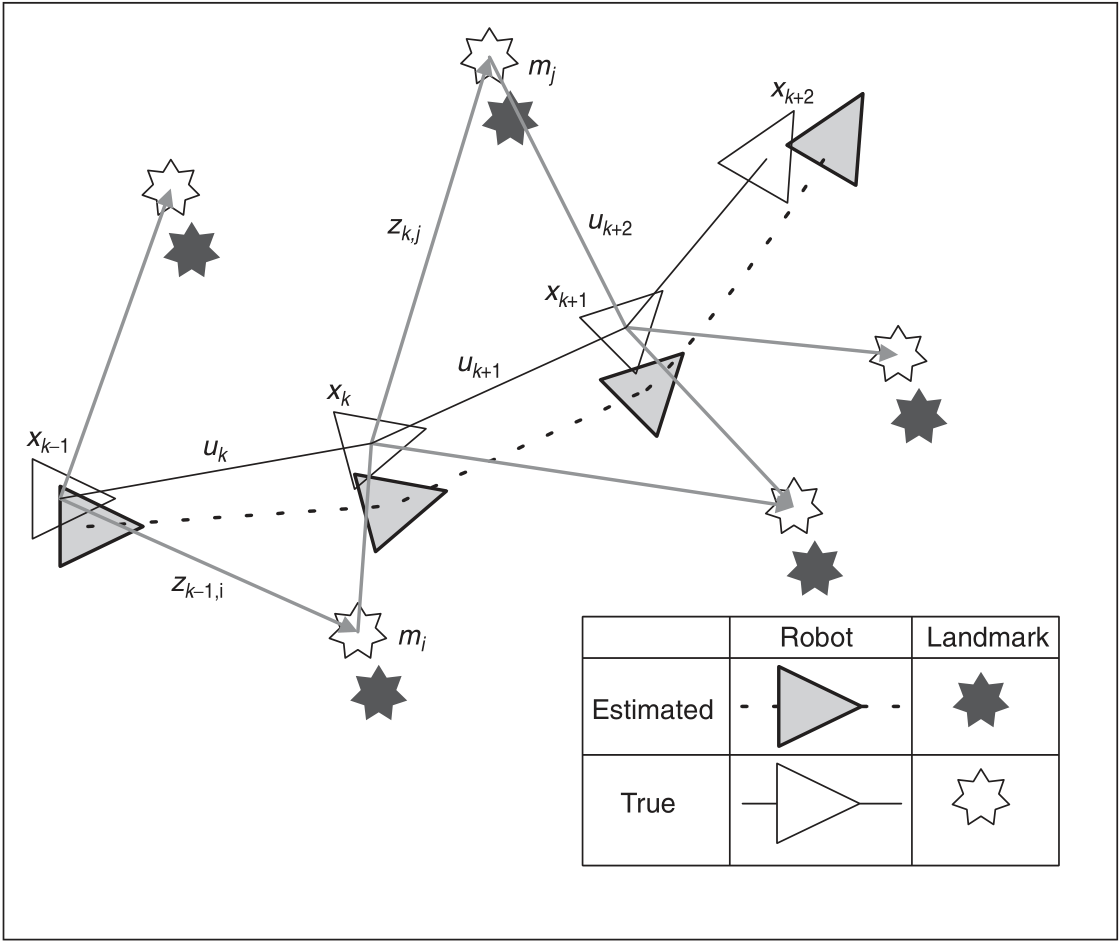
\includegraphics[width=0.60\textwidth]{img/fundamentals/slam.png}
    \caption{The process of SLAM algorithm which estimates the position at the time $k$ by using the measurements to different landmarks\cite{durrant-Whyte2006}}
    \label{fig:slam}
\end{wrapfigure}

The main purpose of mobile mapping systems is to create a new map of an unknown environment with a portable platform.
These platforms can be attached to very small robots but also on bigger cars or even plains, depending on their purpose.
A lot of mobile mapping systems use more than one sensor type to use the advantages of each sensor.
The characteristics of most common sensors for mobile mapping systems are explained in section \ref{sec:messurementPrinciples}.

To create a map it is crucial to know the own position.
The localization can be done either global with the help of \ac{GNSS} or related to a local frame by solving the \ac{SLAM} problem.
While \ac{GNSS} can only be used in environments where satellite connections are possible the \ac{SLAM} algorithm can be used whenever it is possible to collect data about the surrounding.
In \ac{SLAM} the mobile mapping platform collects data from their sensors, stores them as a map while it deduce it's location at the same time.
That location can only be estimated because the sensors only measure the position related to the map and not an absolute position like \ac{GNSS}.
But for that estimation it is not not necessary to know any a priori information of location\cite{durrant-Whyte2006}.

The process of \ac{SLAM} is visualized in figure \ref{fig:slam}.
It shows how the platform estimates the position of it self and the detected landmarks at the time instant $k$ by using the following quantities\cite{durrant-Whyte2006}:

\begin{labeling}{$x_k$}
\item[\boldmath$x_k$] vector describing the pose
\item[\boldmath$u_k$] vector with control information about the movement between $k-1$ and $k$
\item[\boldmath$m_i$] vector with time invariant locations of the $i$th landmark
\item[\boldmath$z_{ik}$] vector with observation of the $i$th landmark at time $k$
\end{labeling}

Together with these vectors the following sets are defined:

\begin{labeling}{\boldmath$X_{0:k}=\{x_0, x_1, x_2, \cdots , x_k\}$}
\item[\boldmath$X_{0:k}=\{x_0, x_1, x_2, \cdots , x_k\}$] vector describing the pose
\item[\boldmath$U_{0:k}=\{u_0, u_1, u_2, \cdots , u_k\}$] vector containing the history of control information
\item[\boldmath$m={m_1, m_2, \cdots, m_n}$] set of landmarks
\item[\boldmath$Z_{0:k}=\{z_0, z_1, z_2, \cdots , z_k\}$] vector with all observations of the landmarks
\end{labeling}

\begin{wrapfigure}[17]{I}{0.60\textwidth}
    \centering
    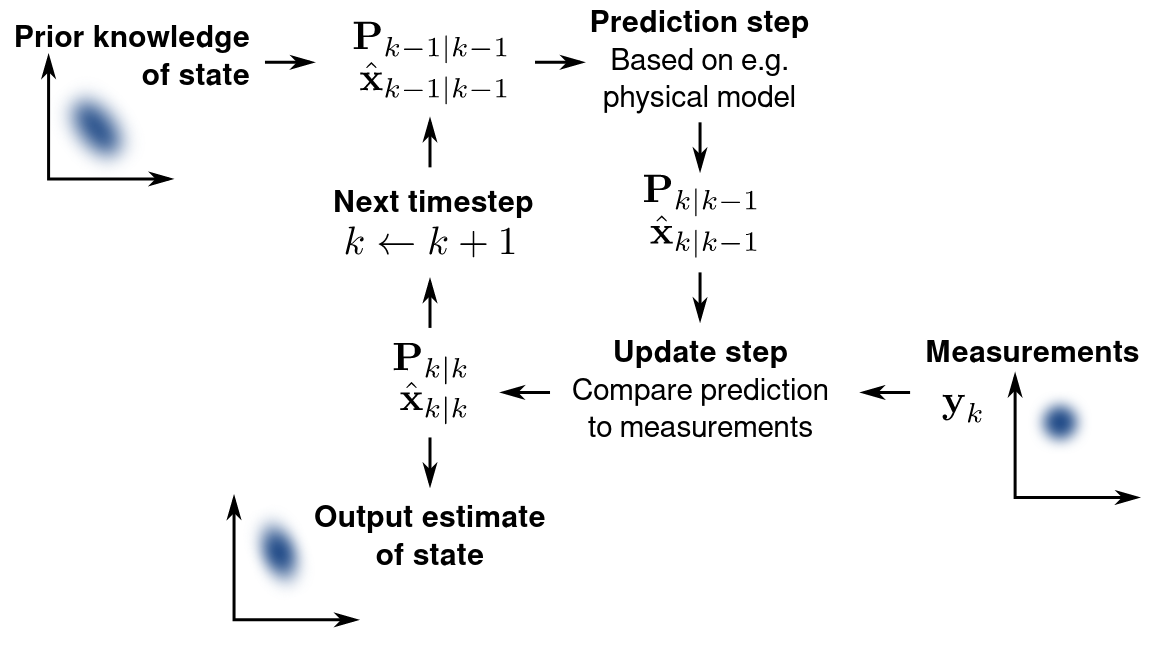
\includegraphics[width=0.60\textwidth]{img/fundamentals/kalmanfilter.png}
    \caption{The basic steps of the Kalman Filter are the prediction and update steps. Beside of the updating the state it also keeps track of the estimated variance\cite{KalmanFilterImage}.}
    \label{fig:kalmanfilter}
\end{wrapfigure}

The results of the SLAM algorithm can be optimised by fusing them with other observations from other sensors.
Typically the Kalman filter or one of the extensions is used to manage the fusion.
The basic Kalman filter is a linear quadratic estimation and because the most physical processes, which are modeled in the filter, are not linear it is not possible to use the Kalman filter with those processes.
But extensions like the extended Kalman filter or the unscented Kalman filter are developed for these applications.

The algorithm can be split in two steps the first step is the prediction step and the second is the update step.
The two steps are executed in a recursive way so that in the prediction step the Kalman filter uses the estimation $\hat{x}$ at the time step $k-1$ together with their uncertainties $P$.
After the prediction based on a physical model the uncertainties $P_{k|k-1}$ and estimation $\hat{x}_{k|k-1}$ are given to the update step.
In the update step the Kalman filter typically adds some random error to the measurements $y_{k}$ and update the estimation using a weighted average.
The results of the update step are  the estimation $\hat{x}_{k|k}$ and the uncertainties $P_{k|k}$ which can be used to determine the quality of the general outcome\cite{Zarchang2000}.

With the random noise, which is mostly a gaussian and the weight the Kalman filter can be tuned to very good results.
Ullah et al.~present the results of simulate a SLAM algorithm with the Kalman filter in a unknown environment and that this method is efficient and viable\cite{Ullah}.

The weights define if there is more trust in the measurement or in the estimation.

\section{Messurement Principles}\label{sec:messurementPrinciples}
Every sensor has different advantages and disadvantages which are caused by physical reasons or because improving would not allow to use them in a cost efficient mobile thermal mapping system.
But the disadvantages can be overcome by using the advantages of other sensors.
Each sensor type is presented on the basis of their fundamental functionality which shows their basic advantages and disadvantages.
The disadvantages can be larger depending on the implementation, manufacturing processes and use cases.

\subsection{LiDAR}\label{ssec:lidar}

\ac{LiDAR} sensors measures the range to a light reflecting object by sending out a pulse of directed light and measure the time until the reflection comes back.
Using a static laser beam allows only getting a range in one direction, but adding one or two movable mirrors allows to scan in two respective three dimensions.

\begin{wrapfigure}[12]{I}{0.55\textwidth}
    \centering
    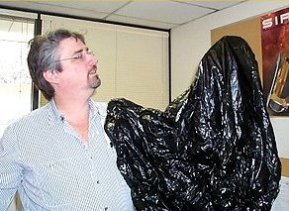
\includegraphics[height=2.8cm]{img/fundamentals/Human-Visible.jpg}
    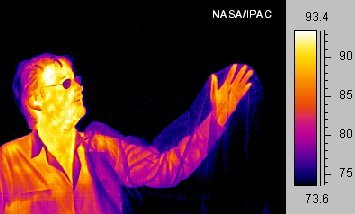
\includegraphics[height=2.8cm]{img/fundamentals/Human-Infrared.jpg}

    \caption{The RGB image in the left and the IR image on the right. The pictures show that IR radiation is blocked by the glasses but not by the thin plastic bag.}
    \label{fig:humanIRVIS}
\end{wrapfigure}

The used light needs to be in a specific spectrum not hurting the eyes and also not visible for human eyes.
It should also be reflected by all materials which can block the mapping platform.

\begin{wrapfigure}[28]{I}{0.45\textwidth}
    \centering
    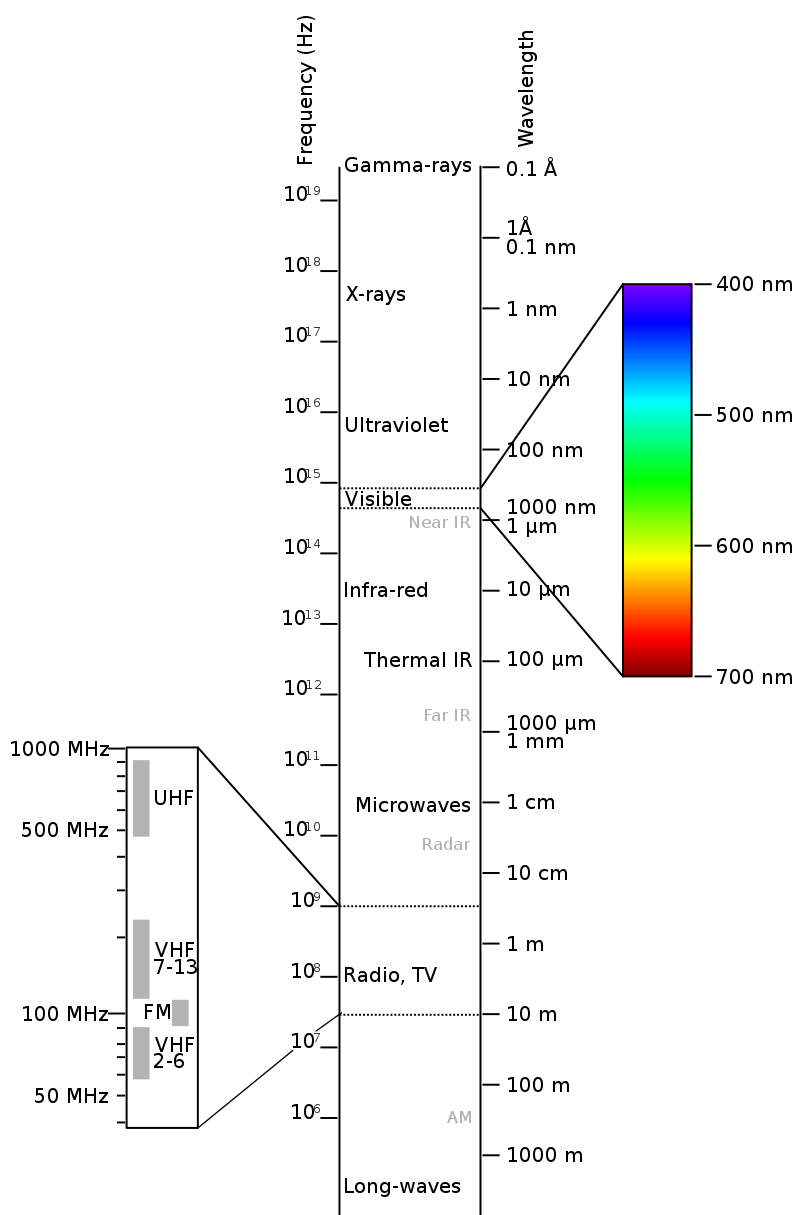
\includegraphics[width=0.45\textwidth]{img/fundamentals/em_spectrum.png}
    \caption{The electromagnetic spectrum with the visible light only covering a small part and the infrared as well as thermal infrared having a smaller frequency \cite{spectrum}
    }
    \label{fig:spectrum}
\end{wrapfigure}

This method is bases on the reflection of the laser but not all materials reflect all of the laser beam which leads to multiple echoes.
The different intensities could also be used for localization\cite{Barsen2018}.

The range measurements are highly accurate but the more dimensions are desired the more time is needed for one full measurement.
E.g. the Z+F PROFILER\circledR{} 9012\cite{z+fLaserProfiler} needs $20.41\si{ms}$ for a 2D scan but the Z+F IMAGER\circledR{} 5016 needs at least $22\si{s}$.

The output of a \ac{LiDAR} sensor depends on the number of dimensions they measure.
All of them measure a distance but for each additional dimension one angle is added.
But in case of 3D scanner the output format is often a 2.5D image.

\subsection{Thermal Camera}\label{ssec:thermalCamera}

Every object emits \ac{EM} radiation which depends on the temperature of the object where the most of these emitted radiation is in the \ac{IR} spectrum.
Using the self emitted radiation has the advantages to be able to take measurements without any other active components like a lamp for classic RGB images.

Unlike RGB cameras thermal cameras doesn't use the \ac{VIS} but the \ac{IR} light.
Both lights can be described as \ac{EM} waves within an other spectrum.
\ac{VIS} covers only a tiny part with wave-lengths from $0.38$ to $0.78\si{\micro m}$, followed at longer wavelengths by the \ac{IR} from $0.78\si{\micro m}$ to $1\si{\milli m}$.
Within the \ac{IR} spectrum the \ac{TIR} is between $8\si{\micro m}$ and $14\si{\micro m}$\cite{Vollmer2017} (Figure \ref{fig:spectrum}).
But the same material can have different characteristics for these two spectrum.
As shown in figure \ref{fig:humanIRVIS} the glasses are blocking the \ac{IR} but the plastic bag not.

Like the common RGB cameras \ac{IR} cameras also use a lense to focus on the observed object and a sensor to transform the \ac{EM} waves in electric signals.
The lenses typically reflect parts of the \ac{IR} radiation which lowers the quality of the result.
To avoid these looses anti reflection coatings, band filters witch are known from the optical spectrum are used\cite{Vollmer2017} but also other materials are used for the lenses.
On the side of sensors there are two types which are used nowadays, the cooled and the uncooled sensors.
Comparing these two types the cooled is more precise but also higher in cost, size and weight.
An other drawback from the cooled sensors is that they need several minutes to cool down before they can take the first images.
Depending on the application the drawbacks can be accepted in favour of the higher precision.

Booth sensors don't measures the frequency, like the RGB sensors, but the intensity of \ac{TIR} radiation which leads to monochromatic images.
These images can be visualized in grey tone or pseudo colored images.

\subsection{Stereo Camera}\label{ssec:stereoCamera}
Stereo Cameras are typical two calibrated high definition RGB cameras observing the same scene.
For mobile mapping systems these two cameras are often arranged at the same horizontal plane with a distance of $10-12\si{cm}$.
This distance is named Baseline $B$.
Due to the distance between the two cameras each of them sees two slightly different pictures with different angles to the observed objects.
Because each cameras picture is distorted, each camera need a intrinsic calibration.
And to calculate the spacial information the cameras need a extrinsic calibration.

After the calibration the pictures can be rectified to proceed with matching single objects in the pictures.
The matching is necessary to calculate the disparity map which represents the depth of each pixel.
The matching between the objects can either be done manual or automatically while the manual matching is only possible in the post processing and the automatically can be used in real-time processing and post processing\cite{Zarchang2000}.

\subsection{IMU}\label{ssec:imu}

A basic \ac{IMU} measures the linear acceleration using accelerometer and gyroscope to detect the rotational rate.
Typically these are measured over three perpendicular axis.
Modern \ac{IMU}s also use magnetometer to measure the heading and barometer to estimate the hight.
With all these information the orientation of the \ac{IMU} can be estimated by fusing them\cite{kim2004}.

\ac{IMU}s tend to drift over the time because even very small errors or noises have a big impact during the integration process.
But the models how to measure the errors of gyroscope and accelerometer are described in detail by Titteron and Weston\cite{titterton2005}.

Even more advanced \ac{IMU}s use \ac{GNSS} to improve their position.
That can be done by direct or indirect integration.
Where the indirect integration uses the measurements of the sensors to integrate them in different aproaches like loosely or tightly coupled or closed/open-loop etc.
In these concepts a extended Kalman filter is typically used which leads to a high demand on computational power due to the persistent calculation of the Kalman gain.
On the other hand the direct integration uses the results of booth sensors as input of a Kalman filter with the advantages that the equations are not as complex as in the indirect method\cite{Qi2002}.

Booth methods of integration can not only be done with \ac{GNSS} but also with the results of the \ac{SLAM} algorithm.

